\section{Trees}
\label{sec:trees}

\nemquote{
}{}

\subsection{Merkle Tree}

A Merkle Tree\cite{Merkle1988} is a tree of hashes that allows efficient existence proofs.
Within \codename, all basic merkle trees are constrained to being balanced and binary.
Each leaf node contains a hash of some data.
Each non-leaf node is constructed by hashing the hashes stored in child nodes.
In the \codenamespace implementation, when any (non-root) layer contains an odd number of hashes, the last hash is doubled when calculating the parent hash.

\begin{figure}[h]
	\begin{center}
		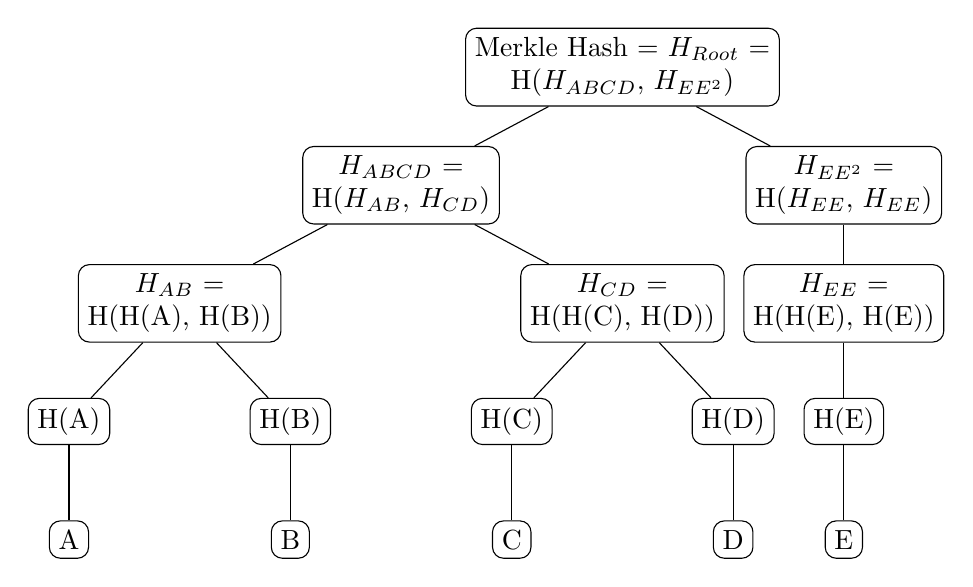
\begin{tikzpicture}[every node/.style = {shape=rectangle, rounded corners, draw, align=center}]]
			\tikzstyle{level 3}=[sibling distance=8em]
			\node {Merkle Hash = $H_{Root}$ =\\H($H_{ABCD}$, $H_{EE^2}$)}
				child [sibling distance=16em] { node {$H_{ABCD}$ =\\H($H_{AB}$, $H_{CD}$)}
					child { node {$H_{AB}$ =\\H(H(A), H(B))}
						child { node {H(A)} { child { node {A} } } }
						child { node {H(B)} { child { node {B} } } }
					}
					child { node {$H_{CD}$ =\\H(H(C), H(D))}
						child { node {H(C)} { child { node {C} } } }
						child { node {H(D)} { child { node {D} } } }
					}
				}
				child [sibling distance=16em] { node {$H_{EE^2}$ =\\H($H_{EE}$, $H_{EE}$)}
					child { node {$H_{EE}$ =\\H(H(E), H(E))}
						child { node {H(E)} { child { node {E} } } }
					}
				};
		\end{tikzpicture}
		\caption{Four level Merkle tree composed of five data items}
	\end{center}
\end{figure}

\begin{figure}
	\begin{center}
		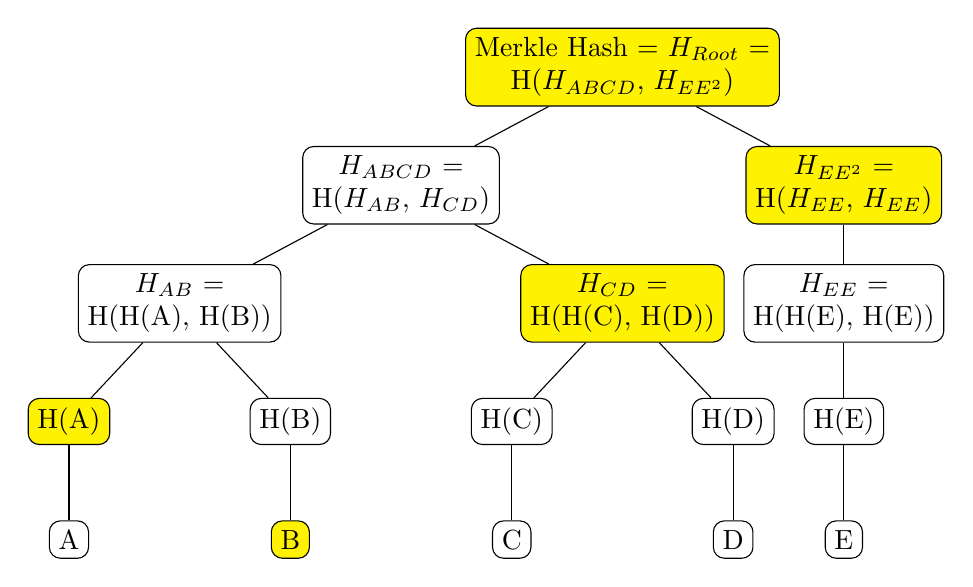
\begin{tikzpicture}[every node/.style = {shape=rectangle, rounded corners, draw, align=center}]]
			\tikzset{ highlight/.style = {fill = yellow} }
			\tikzstyle{level 3}=[sibling distance=8em]
			\node [highlight] {Merkle Hash = $H_{Root}$ =\\H($H_{ABCD}$, $H_{EE^2}$)}
				child [sibling distance=16em] { node {$H_{ABCD}$ =\\H($H_{AB}$, $H_{CD}$)}
					child { node {$H_{AB}$ =\\H(H(A), H(B))}
						child { node [highlight] {H(A)} { child { node {A} } } }
						child { node {H(B)} { child { node [highlight] {B} } } }
					}
					child { node [highlight] {$H_{CD}$ =\\H(H(C), H(D))}
						child { node {H(C)} { child { node {C} } } }
						child { node {H(D)} { child { node {D} } } }
					}
				}
				child [sibling distance=16em] { node [highlight] {$H_{EE^2}$ =\\H($H_{EE}$, $H_{EE}$)}
					child { node {$H_{EE}$ =\\H(H(E), H(E))}
						child { node {H(E)} { child { node {E} } } }
					}
				};
		\end{tikzpicture}
		\caption{Merkle proof required for proving existence of B in the tree}
	\end{center}
\end{figure}

A benefit of using merkle trees is that the existence of a hash in a tree can be proven with only $\log(N)$ hashes.
This allows for existence proofs with relatively low bandwidth requirements.

A merkle proof for existence requires a single hash from each level of the tree.
In order to prove the existence of $B$, a client must:
\begin{enumerate}
	\item{Calculate $H(B)$}
	\item{Obtain $H_{Root}$; in \codename, this is stored in the block header}
	\item{Request $H(A)$, $H_{CD}$, $H_{EE^2}$}
	\item{Calculate $H_{Root'} = H(H(H(H(A), H(B)), H_{CD}), H_{EE^2})$}
	\item{Compare $H_{Root}$ and $H_{Root'}$; if they match $H(B)$ must be stored in the tree}
\end{enumerate}

\subsection{Patricia Tree}

A patricia tree is a deterministically ordered tree.
It is constructed from key value pairs, and supports both existence and non-existence proofs requiring only $\log(N)$ hashes.
Non-existence proofs are possible because this tree is deterministically sorted by keys.
The application of the same data, in any order, will always result in the same tree.

When inserting a new key value pair into the tree, the key is decomposed into nibbles and each nibble is logically its own node in the tree.
All keys within a single tree are required to have the same length, which allows slightly optimized algorithms.

For illustration, consider the following key value pairs in \autoref{treesExampleData}.
Some examples will use ASCII keys to more clearly elucidate concepts, while others will use hex keys to more accurately depict \codenamespace implementations.

\autoref{treesAsciiExpanded} depicts a full patricia tree where each letter is represented by a separate node.
Although this tree is logically correct, it is quite expansive and uses a lot of memory.
A typical key is a 32 byte hash value, which implies that storing a single value could require up to 64 nodes!
In order to work around this limitation, successive empty branch nodes can be collapsed into either a branch node with at least two connections or a leaf node.
This leads to a different but more compact tree, as depicted in \autoref{treesAsciiCompact}.

\begin{table}[ht]
	\begin{center}
		\begin{tabular}{|c|c|c|}
			\hline
			key & hex-key & value \\
			\hline
			do** & \texttt{646F0000} & verb \\
			dog* & \texttt{646F6700} & puppy \\
			doge & \texttt{646F6765} & mascot \\
			hors & \texttt{686F7273} & stallion \\
			\hline
		\end{tabular}
		\caption{Patricia tree example data}
		\label{treesExampleData}
	\end{center}
\end{table}

\begin{figure}[H]
	\begin{center}
		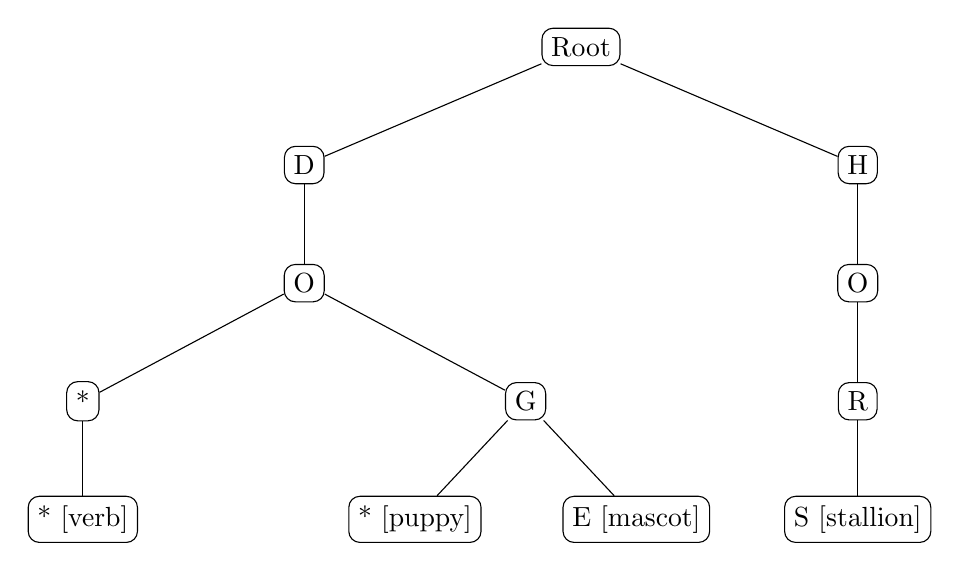
\begin{tikzpicture}[every node/.style = {shape=rectangle, rounded corners, draw, align=center}]]
			\tikzstyle{level 1}=[sibling distance=20em]
			\tikzstyle{level 3}=[sibling distance=16em]
			\tikzstyle{level 4}=[sibling distance=8em]
			\node {Root}
				child { node {D}
					child { node {O}
						child { node {*}
							child { node {* [verb]} }
						}
						child { node {G}
							child { node {* [puppy]} }
							child { node {E [mascot]} }
						}
					}
				}
				child { node {H}
					child { node {O}
						child { node {R}
							child { node {S [stallion]} }
						}
					}
				};
		\end{tikzpicture}
		\caption{Conceptual (expanded) patricia tree composed of four data items}
		\label{treesAsciiExpanded}
	\end{center}
\end{figure}

\begin{figure}[H]
	\begin{center}
		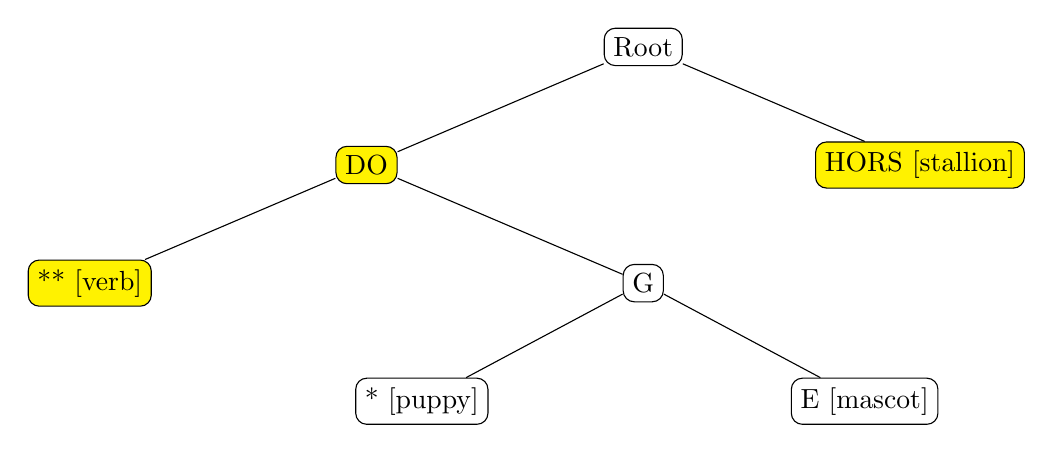
\begin{tikzpicture}[every node/.style = {shape=rectangle, rounded corners, draw, align=center}]]
			\tikzset{ highlight/.style = {fill = yellow} }
			\tikzstyle{level 1}=[sibling distance=20em]
			\tikzstyle{level 3}=[sibling distance=16em]
			\tikzstyle{level 4}=[sibling distance=8em]
			\node {Root}
				child { node [highlight] {DO}
					child { node [highlight] {** [verb]} }
					child { node {G}
						child { node {* [puppy]} }
						child { node {E [mascot]} }
					}
				}
				child { node [highlight] {HORS [stallion]} };
		\end{tikzpicture}
		\caption{Conceptual (compact) patricia tree composed of four data items}
		\label{treesAsciiCompact}
	\end{center}
\end{figure}

\subsection{Merkle Patricia Tree}

A merkle patricia tree is a combination of merkle and patricia trees.
The \codenamespace implementation centers around two types of nodes: leaf nodes and branch nodes.
Each leaf node contains a hash of some data.
Each branch node contains up to sixteen pointers to child nodes.

Like in a basic merkle tree, each merkle patricia tree has a root hash.
Unlike in a basic merkle tree, the hashes stored in the tree are a bit more complex.

Every node in the tree has a tree node path.
This path is composed of a sentinel nibble followed by zero or more path nibbles.
If the path represents a leaf node, $\texttt{0x2}$ will be set in the sentinel nibble.
If the path is composed of an odd number of nibbles, $\texttt{0x1}$ will be set in the sentinel nibble and the second nibble will contain the first path nibble.
If the path is composed of an even number, the second nibble will be set to $\texttt{0x0}$ and the second byte will contain the first path nibble.

\begin{figure}[ht]
	\begin{center}
		\begin{tikzpicture}[node distance=-\pgflinewidth]
			% odd tree node path
			\node[anchor=center] (lbl1) {odd path};
			\node[crecb,right=0.25cm of lbl1] (bit11) {\texttt{0}};
			\node[crecb,right=of bit11] (bit12) {\texttt{0}};
			\node[crecb,right=of bit12] (bit13) {$b_{leaf}$};
			\node[crecb,right=of bit13] (bit14) {\texttt{1}};

			\node[crecb,right=of bit14] (nibble12) {$nibble_1$};
			\node[crecb,right=of nibble12] {$nibble_2..nibble_{N [odd]}$};

			\node[fit=(bit11)(bit12)(bit13)(bit14), draw, dotted, rounded corners] (nibble11) {};
			\draw[decorate,decoration={brace,raise=2pt},very thick] (nibble11.north west) -- node[above=4pt] {sentinel nibble} (nibble11.north east);

			\node[fit=(nibble11)(nibble12), draw, dotted, rounded corners] (byte11) {};
			\draw[decorate,decoration={brace,mirror,raise=2pt},very thick] (byte11.south west) -- node[below=4pt] {byte 1} (byte11.south east);

			% even tree node path
			\node[anchor=center, below=2.5cm of lbl1] (lbl2) {even path};
			\node[crecb,right=0.25cm of lbl2] (bit21) {\texttt{0}};
			\node[crecb,right=of bit21] (bit22) {\texttt{0}};
			\node[crecb,right=of bit22] (bit23) {$b_{leaf}$};
			\node[crecb,right=of bit23] (bit24) {\texttt{0}};

			\node[crecb,right=of bit24] (nibble22) {\texttt{0000}};
			\node[crecb,right=of nibble22] {$nibble_1..nibble_{N [even]}$};

			\node[fit=(bit21)(bit22)(bit23)(bit24), draw, dotted, rounded corners] (nibble21) {};
			\draw[decorate,decoration={brace,raise=2pt},very thick] (nibble21.north west) -- node[above=4pt] {sentinel nibble} (nibble21.north east);

			\node[fit=(nibble21)(nibble22), draw, dotted, rounded corners] (byte21) {};
			\draw[decorate,decoration={brace,mirror,raise=2pt},very thick] (byte21.south west) -- node[below=4pt] {byte 1} (byte21.south east);
		\end{tikzpicture}
		\caption{Tree node path encoding}
	\end{center}
\end{figure}

A \emph{leaf node}\index{node!leaf} is composed of the following two items:
\begin{enumerate}
	\item{TreeNodePath: Encoded tree node path (with leaf bit set).}
	\item{ValueHash: Hash of the value associated with the key ending at the leaf.}
\end{enumerate}

The hash of a leaf node can be calculated by hashing its component parts: $$\textit{H(Leaf)}=H(TreeNodePath, ValueHash)$$.

A \emph{branch node}\index{node!branch} is composed of the following items:
\begin{enumerate}
	\item{TreeNodePath: Encoded tree node path (with leaf bit unset).}
	\item{$LinkHash_{0...15}$: Hashes of children where the index is the next nibble part of the path.
	When no child is present at an index, a zero hash should be used instead.}
\end{enumerate}

The hash of a branch node can be calculated by hashing its component parts: $$\textit{H(Branch)}=H(TreeNodePath, LinkHash_0,..LinkHash_{15})$$.

Reconstructing the earlier example with hex keys yields a tree that illustrates a more accurate view of how a \codenamespace tree is constructed.
Notice that each branch node index composes a single nibble of the path.
This is depicted in \autoref{treesHexCompact}.

\begin{figure}[ht]
	\begin{center}
		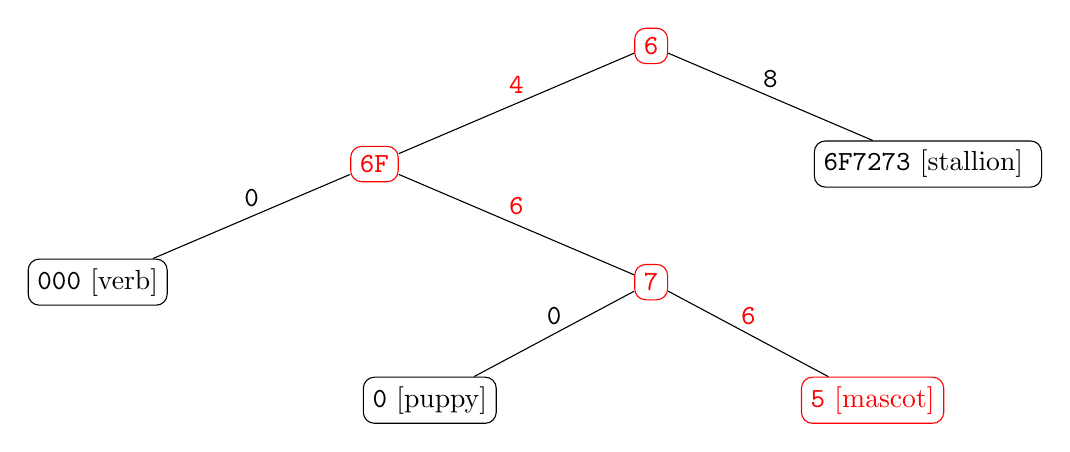
\begin{tikzpicture}
			\begin{scope}[every node/.style = {shape=rectangle, rounded corners, draw, align=center}]
				\tikzstyle{level 1}=[sibling distance=20em]
				\tikzstyle{level 3}=[sibling distance=16em]
				\tikzstyle{level 4}=[sibling distance=8em]
				\node (6) [red] {\texttt{6}}
					child { node (646F) [red] {\texttt{6F}}
						child { node (646F0000) {\texttt{000} [verb]} }
						child { node (646F67) [red] {\texttt{7}}
							child { node (646F6700) {\texttt{0} [puppy]} }
							child { node (646F6765) [red] {\texttt{5} [mascot]} }
						}
					}
					child { node (686F7273) {\texttt{6F7273} [stallion] } };
			\end{scope}

			\path (6) -- (646F) node [red, above, pos=0.5] {{\texttt{4}}};
			\path (6) -- (686F7273) node [above, pos=0.5] {\texttt{8}};
			\path (646F) -- (646F0000) node [above, pos=0.5] {\texttt{0}};
			\path (646F) -- (646F67) node [red, above, pos=0.5] {{\texttt{6}}};
			\path (646F67) -- (646F6700) node [above, pos=0.5] {\texttt{0}};
			\path (646F67) -- (646F6765) node [red, above, pos=0.5] {{\texttt{6}}};
		\end{tikzpicture}
		\caption{
			Realistic patricia tree with branch and leaf nodes and all optimizations.
			Path to $mascot$ [\texttt{646F6765}] is highlighted.
		}
		\label{treesHexCompact}
	\end{center}
\end{figure}

\subsection{Merkle Patricia Tree Proofs}

A merkle proof for existence requires a single node from each level of the tree.
In order to prove the existence of $\{key = \texttt{646F6765}, value = H(mascot)\}$, a client must:
\begin{enumerate}
	\item{Calculate $H(mascot)$ (remember, all leaf values are hashes).}
	\item{Request all nodes on the path $\texttt{646F6765}$: $Node_{6}$, $Node_{646F}$, $Node_{646F67}$.}
	\item{Verify that $Node_{646F67}::Link[6]$ is equal to $H(Leaf(mascot))$.}
	\item{Calculate $H(Node_{646F67})$ and verify that $Node_{6467}::Link[6]$ is equal to $H(Node_{646F67})$.}
	\item{Calculate $H(Node_{6467})$ and verify that $Node_{6}::Link[4]$ is equal to $H(Node_{6467})$.}
	\item{Existence is proven if all calculated and actual hashes match.}
\end{enumerate}

A merkle proof for non-existence requires a single node from each level of the tree.
In order to prove the non-existence of $\{key = \texttt{646F6764}, value = H(mascot)\}$, a client must:
\begin{enumerate}
	\item{Calculate $H(mascot)$ (remember, all leaf values are hashes).}
	\item{Request all nodes on the path $\texttt{646F6764}$: $Node_{6}$, $Node_{646F}$, $Node_{646F67}$.}
	\item{
		Verify that $Node_{646F67}::Link[5]$ is equal to $H(Leaf(mascot))$.
		Since $Link[5]$ is unset, this check will fail.
		If the value being searched for was in the tree, it must be linked to by this node because of the determinism of the tree.
	 }
\end{enumerate}
